\graphicspath{{NeutrinoSearches/Figures/}}

\chapter{Heavy Neutrino Searches}\label{chapter: neutrinoSearches}

\section{Neutrino Searches in the LHC}

Heavy neutrino searches in the LHC have mainly focused in production via Drell-Yan mechanism. The Feynman diagram for this process is shown in Figure \ref{fig: HN_DY}. As shown in the diagram, the heavy neutrino results from  a W boson that decays into a lepton and the heavy neutrino. In this model, the heavy neutrino decays into a lepton and a W boson. The latter decays into two quarks that result in two jets observed by the detector. Advances in the collision energies provided by the LHC have allowed probing for masses of heavy neutrino at larger scales. This fact is shown in Figure \ref{fig: LHCvsTevatron} where a comparison in the cross section of the Drell-Yan heavy neutrino process in the Tevatron and the LHC is shown. It can be seen clearly that the LHC, due to its higher center of mass energy in the collision, has a greater cross section than the one present at the Tevatron for the same process \cite{Tevatron}.


\begin{figure}[H]
\centering
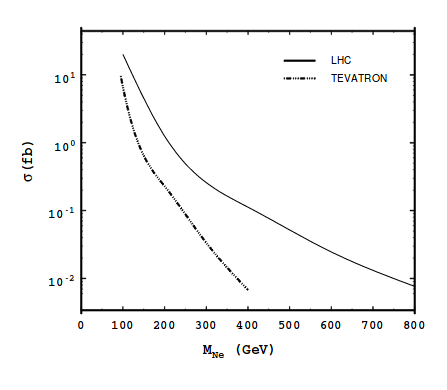
\includegraphics[width=\linewidth]{LHCvsTevatron}
\caption{Cross sections for heavy neutrino production at the LHC and the Tevatron (Taken from \cite{Tevatron})}
\label{fig: LHCvsTevatron}
\end{figure}


As mentioned in \cite{HNDrell-Yan}, the process mentioned above is the dominant signal for a heavy neutrino with a mass between the 100 GeV and 500 GeV. The main problem with this type of process is that, given there is a W boson in the heavy neutrino production, the cross section for large values of the heavy neutrino mass decreases rapidly. The fast decrease in the signal cross section can be observed in Figure \ref{fig: LHCvsTevatron}. This small cross section rises a problem to experimentally observe a signal with a heavy neutrino mass greater than 400 GeV \cite{HNDrell-Yan}.

Although the production of heavy neutrino through the Drell-Yan process has a small cross section, it has the advantage of having a clean signal if the heavy neutrino has a decay of the form $N \rightarrow l^{\pm} W^{\mp} \rightarrow l^{\pm} jj$ \cite{HNDrell-Yan}. This type of process allows the detection of all the products of the final state of the process. That is, signal from the two leptons and the two jets that result at the end of the process should be observed in the detector. 

\begin{figure}[H]
\centering
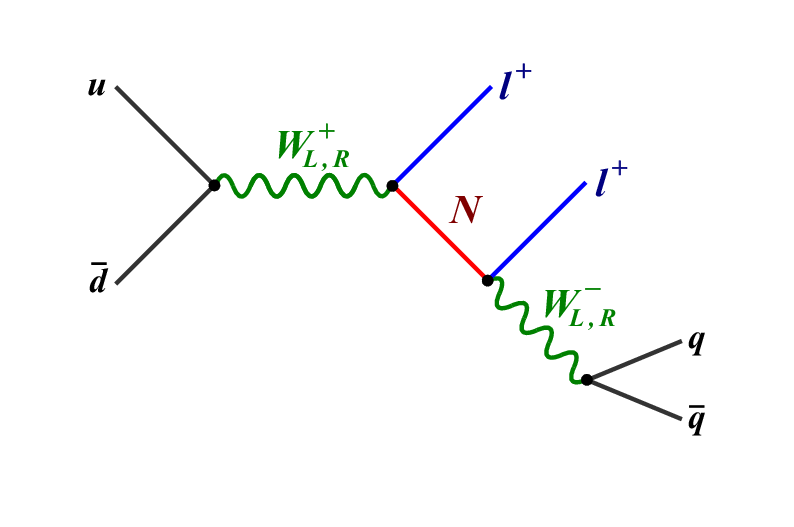
\includegraphics[width=\linewidth]{Feynman_HN_DY}
\caption{Feynman diagram of heavy neutrino production by Drell-Yan process}
\label{fig: HN_DY}
\end{figure}

As noted in \cite{See-saw}, all the heavy neutrino searches in the LHC have focused in the Drell-Yan process. It is also mentioned that studies involving final states with taus have not been explored because of the challenges of reconstructing and tagging correctly a $\tau$. However, it is also mentioned that this can be solved with the improvement of $\tau$-tagging algorithms. The latter makes a study like the one presented in this monograph novel, because of the inclusion of taus instead of muons and electrons in the final state.   

\section{Heavy Neutrino Search with Vector Boson Fusion}

The first difference between most of the studies mentioned in the previous section and the one done in this study is the use of $\tau$ instead of $\mu$ for the lepton in the the process. The second, and main difference, is the use of the Vector Boson Fusion technique. As stated earlier, neutrino searches have been mainly performed using the Drell-Yan mechanism shown in Figure \ref{fig: HN_DY}. However, a search using the Vector Boson Fusion, or VBF, technique has not been conducted. The main difference between the Drell-Yan process and the one including the VBF topology is the addition of two jets resulting from the fusion of two bosons. These two jets would have the characteristic of traveling in opposite directions and in the longitudinal region of the detector when they are created. As a result, the VBF topology includes two jets with a big angular separation in the detector, because they should be detected in opposite hemispheres (high $\Delta \eta$ separation) and in the endcap region (large $\eta$ values). Also, the jets coming from the Vector Boson Fusion process would typically have greater transverse momentum $p_{T}$ than jets coming from, for example, the quarks resulting from the decay of bosons. These characteristics mentioned above would allow to identify these jets coming from the VBF process, hence increasing the possibility of identifying the signal from experimental noise in the detector.

The addition of Vector Boson Fusion to the Drell-Yan process of the heavy neutrino would result in Feynman diagrams like the ones shown in Figures \ref{fig: hnZ} and \ref{fig: hnGamma}. Figure \ref{fig: hnZ} shows the production of a heavy neutrino including the fusion of boson Z with boson W, and Figure \ref{fig: hnGamma} shows the fusion of boson gamma, or photon, with boson W. These two examples show that the bosons that fuse in the VBF processes can be multiple combinations of vector bosons. Also, it is noteworthy that the Feynman diagram portion regarding the production of the heavy neutrino remains unchanged compared to the one of the Drell-Yan production process shown in Figure \ref{fig: HN_DY}. The latter shows how the Vector Boson Fusion is an addition to the process that would help with the identification of the signal, but does not affect the original process that is being studied. The final states for the processes shown in these two diagrams would include two jets coming from the VBF process, two $\tau$'s, and two jets coming from the quarks resulting of the $W^{-}$ decay

\begin{figure}[H]
\centering
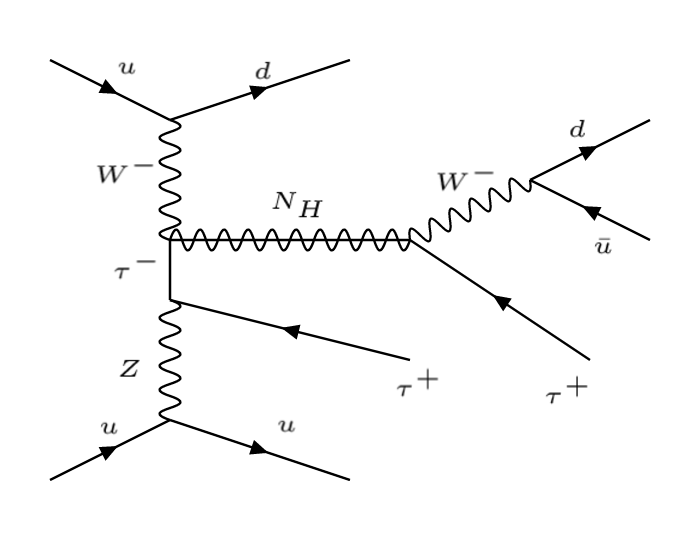
\includegraphics[scale = 0.45]{Figures/Feynman_hnZ}
\caption{Feynman diagram of heavy neutrino production including VBF and involving Z boson}
\label{fig: hnZ}
\end{figure}

\begin{figure}[H]
\centering
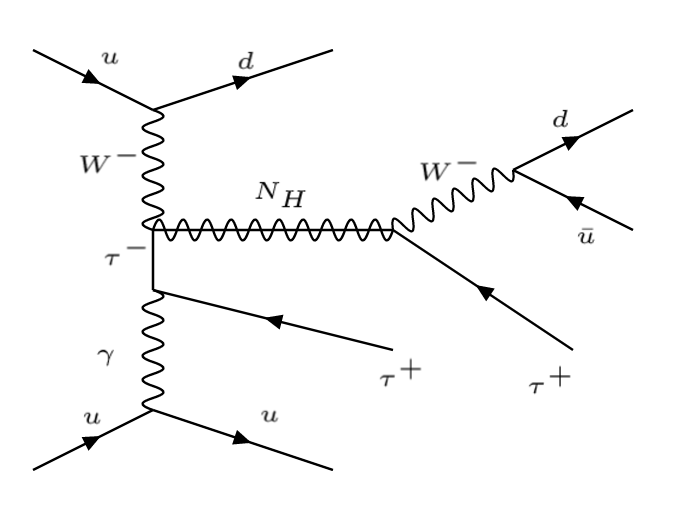
\includegraphics[scale = 0.45]{Figures/Feynman_hnGamma}
\caption{Feynman diagram of heavy neutrino production including VBF and involving photon}
\label{fig: hnGamma}
\end{figure}


A search using the VBF topology would be promising, because there could be a potential enhancement of the signal cross section compared with the heavy neutrino production via Drell-Yan process. A comparison of the cross section of both processes is shown in Figure \ref{fig: DY vs VBF}. Although in both cases the cross section decreases when the mass of the heavy neutrino increases, the cross section of the VBF process decay is slower than the one of the Drell-Yan process. This causes that from a value for the heavy neutrino mass of approximately 1.4 TeV the VBF process has a greater cross section compared to the cross section of the heavy neutrino produced by the Drell-Yan process. This plot shows clearly why it is relevant to perform the analysis of a potential search of heavy neutrinos at the LHC using the Vector Boson Fusion technique. Furthermore, this new production model allows to study the couplings of heavy neutrinos to vector bosons. If couplings of heavy neutrinos to quarks are weak, this might be the only production mechanism available to detect heavy neutrinos. In addition, VBF allows a reduction in 3-4 orders of magnitude the presence of background events from Quantum-Chromo-Dynamic events, referred to as QCD. QCD events is one of the largest backgrounds in experimental searches with hadronically decaying taus. 

\begin{figure}[H]
\centering
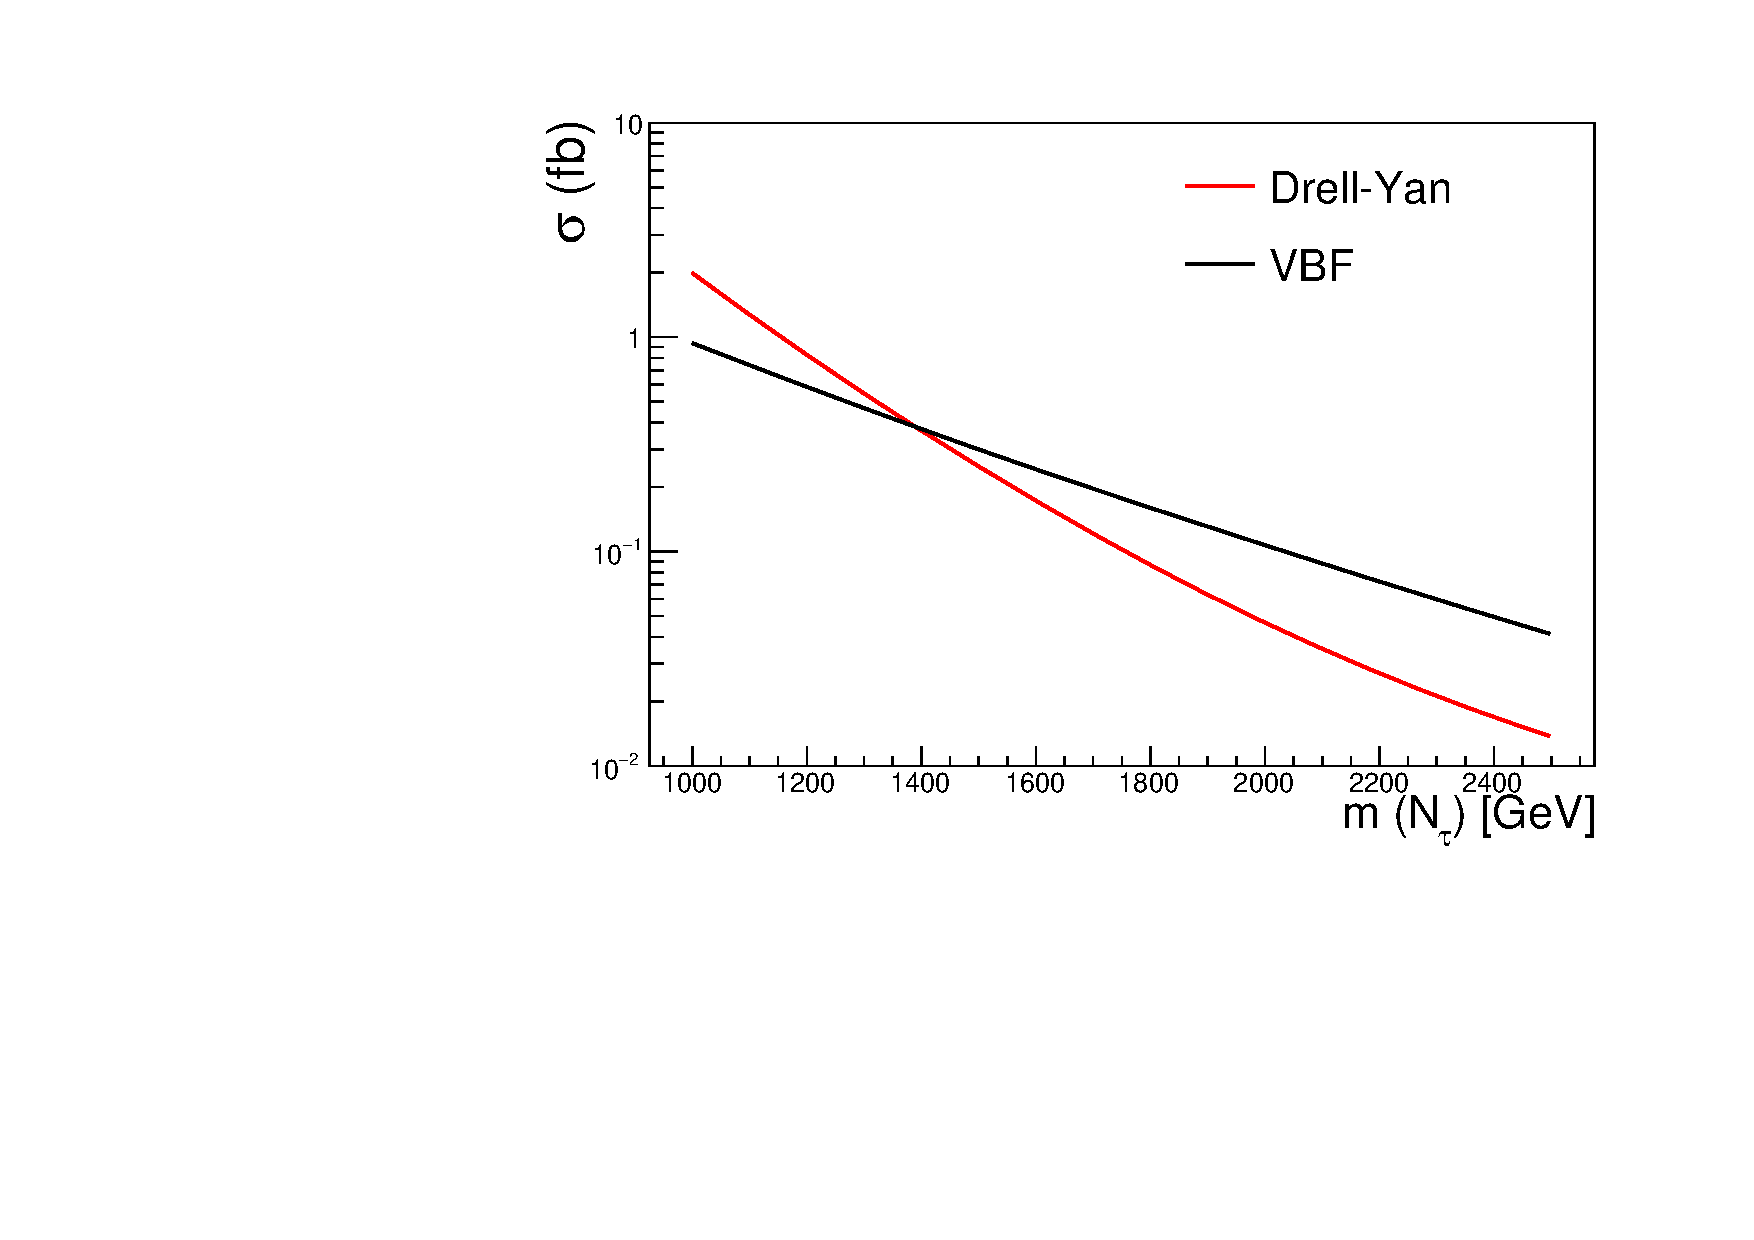
\includegraphics[width=\linewidth]{DY_vs_VBF_HN}
\caption{Feynman diagram of heavy neutrino production by Drell-Yan process}
\label{fig: DY vs VBF}
\end{figure}

